% WHERE THIS GOES. paper/sections/06-thermal.tex, paragraph "\paragraph{Gravitational colour.}".
% Keep that paragraph's opening (Eq. alpha's validity, Re eta(omega), Maxwell's model, Eq. maxwell, and honey), up to
% and including "rearrangement is frozen, and honey need not outshine water at all.", and REPLACE the rest of the
% paragraph, which reads exactly
%
%   In dense
%   matter the friction at those frequencies comes from much faster processes, and
%   an order-of-magnitude guess is $10^{-4}$ to $10^{-3}\,\mathrm{Pa\,s}$, which is
%   why we use $10^{-3}\,\mathrm{Pa\,s}$ as a placeholder. A crystal has no sound
%   waves above its Debye frequency, so above its Debye temperature its glow grows
%   more slowly than $T^3$ as well. Maxwell's model falls steadily with
%   frequency; a real material can have resonances in its losses, and then needs
%   its own spectrum of stress fluctuations, which may exceed this estimate in a
%   band. The spectrum of the glow therefore records a
%   material's mechanical losses, a kind of gravitational colour, and with a
%   frequency-dependent friction the number emissivity must be computed as
%   $j_N = \int \alpha(\omega)\,B_\omega\,\dd\omega/\hbar\omega$ rather than by
%   dividing the power by $2.70\,k_BT$.
%
% by the text below (from "In dense matter" to the end of the file), which keeps its last sentence, on j_N.
% The paragraph that follows in the section, "Two consequences follow. ...", stays as it is. The table and the
% figure* are new floats; place them near this paragraph.
%
% Also: paper/drafts/materials.bib holds the new BibTeX entries (no key is in paper/refs.bib); the figure is
% paper/figures/materials.pdf (and .svg), drawn by paper/figures/fig_materials.py; every number below comes from
% reference/gravcam/materials.py and is checked by reference/tests/test_materials.py. Once merged, the item
% "the friction of real materials at the frequencies of heat, which sets their gravitational colour;" can leave
% the list in sections/12-status.tex.

In dense matter the friction at those frequencies comes from much faster
processes. A wave's wavenumber is about $10^{-5}$ of that of a sound wave of the
same frequency, so it shears a material uniformly and cannot make a single
sound quantum inside it, which is why a lossless solid absorbs only at its
surface. By the
fluctuation--dissipation theorem $\mathrm{Re}\,\eta(\omega)$ is the spectrum of
the material's stress at zero wavenumber, and causality fixes its integral
\cite{SrivastavaWidomPizzella2003}:
\begin{equation}\label{eq:friction-sum}
\frac{2}{\pi}\int_0^\infty \mathrm{Re}\,\eta(\omega)\,\dd\omega = G_\infty - G_0 ,
\end{equation}
the part of the stiffness against shear that relaxes. Here $G_\infty$ resists a
shear too fast for the atoms and the free electrons to follow, and $G_0$ a slow
one; for Maxwell's model the integral is $G_\infty$. At the frequencies of heat
the friction is roughly the stiffness that relaxes there divided by the band
over which it does so (Table~\ref{tab:materials}, Figure~\ref{fig:materials}).

\emph{Free electrons.} In a metal a shear deforms the electrons' Fermi sphere,
and collisions relax it in a time $\tau$:
$\mathrm{Re}\,\eta = \tfrac15 n m v_F^2\,\tau/(1 + \omega^2\tau^2)$, with $n$ the
density of conduction electrons, $m$ their mass and $v_F$ their Fermi speed. The
weight, $\tfrac25 nE_F$, is $38\,\mathrm{GPa}$ in copper, and with its collision
time, $2.5\times10^{-14}\,\mathrm{s}$ \cite{Hirayama2011}, $\omega\tau$ is about
one at the frequencies of heat, where the electrons rub most: whatever $\tau$,
the friction cannot exceed $\tfrac1{10}\,nmv_F^2/\omega$. We give that bound for
iron, whose electrons are not free.

\emph{Driven vibrations.} In a crystal with two atoms in its cell a uniform
shear pushes one set of atoms against the other \cite{Tanner2021}, and so drives
the optical vibration seen in Raman scattering. Silicon glows in a line at
$520\,\mathrm{cm^{-1}}$ ($15.6\,\mathrm{THz}$), where its friction,
$0.03\,\mathrm{Pa\,s}$, is thirty times the placeholder. The line's weight is the
stiffness the shear loses when the atoms relax, $M\omega_0^2\zeta^2/8a =
30\,\mathrm{GPa}$, with $M$ the atomic mass, $\omega_0$ the line, $a$ the cubic
lattice constant and $\zeta$ Kleinman's parameter. In a glass, disorder lets a
uniform shear drive every vibration \cite{LemaitreMaloney2006,Damart2017}; in
silica the weight is about the shear modulus \cite{Leonforte2006}, spread over
the band below $27\,\mathrm{THz}$. In water the stretching of hydrogen bonds near
$8\,\mathrm{THz}$ and the rocking of the molecules carry it \cite{Schulz2020}:
the friction there, $2\times10^{-4}\,\mathrm{Pa\,s}$, is a third of the steady
viscosity.

\emph{Pairs of phonons.} Even in a harmonic crystal the uniform part of the
stress is quadratic in the atoms' displacements $\mathbf u$: integrated over the
volume it is $\tfrac12\,\dd^2/\dd t^2 \sum m u_x u_y$, summed over the atoms,
which oscillates at sums of two phonon frequencies. A wave thus makes and
unmakes pairs of phonons of opposite momentum, up to twice the highest phonon
frequency. This weak channel, of classical weight $2nk_BT$ with $n$ the number of
atoms per volume, about a gigapascal at room temperature, is the only one in an
insulating crystal with one atom in its cell; anharmonicity changes it by a
factor of order one, and it makes an eighth of diamond's glow. Akhiezer's
damping of sound, the relaxation of the thermal phonons in a time $\tau$, puts a
similar weight near zero frequency; at the frequencies of heat its tail is
smaller than the pair band by about $\omega_D\tau$, a thermal phonon's quality
factor.

At room temperature these materials glow at one to sixty per cent of the
placeholder's power (Table~\ref{tab:materials}): $10^{-3}\,\mathrm{Pa\,s}$ is an
upper estimate, and $10^{-4}\,\mathrm{Pa\,s}$ is typical. In every solid larger
than $30\,\mathrm{nm}$ the volume outshines the glow of a lossless surface,
Eq.~\eqref{eq:surface-glow} below. A person, taken as 70 litres of water at
$310\,\mathrm{K}$, radiates $9\times10^{-37}\,\mathrm{W}$: one graviton in
$2\times10^{8}$ years. Metals and water glow redder than a constant friction would; silicon glows in its line, and
diamond, whose line lies in the Wien tail, glows bluer. The spectrum of the glow
therefore records a material's mechanical losses, a kind of gravitational
colour, and with a frequency-dependent friction the number emissivity must be
computed as $j_N = \int \alpha(\omega)\,B_\omega\,\dd\omega/\hbar\omega$ rather
than by dividing the power by $2.70\,k_BT$. When a metal's collision rate is proportional to temperature, as it is above the
Debye temperature \cite{Duthil2014}, $\omega\tau$ at the peak of the glow stays
fixed and the friction falls as $1/T$, so the power grows as $T^3$ and the
number of gravitons as $T^2$: by this estimate the hot iron of
Figure~\ref{fig:closed-furnace} sends about 25 times as many gravitons as the
cold, not more than a hundred.

These estimates hold to about a factor of two: the Drude form ignores that the
collision rate depends on frequency once $\hbar\omega$ exceeds the phonon
energies, Debye's spectrum smooths the peaks of the real one, the glass's weight
assumes that shear relaxes as uniaxial strain does in simulation
\cite{Leonforte2006}, and the water spectrum comes from a classical simulation of
rigid molecules \cite{Schulz2020}. Quartz, with many atoms in its cell, should be
driven like the glass \cite{Damart2017}, and with it most rock; soft tissue
should glow like water.

\begin{table}
\centering
\begin{tabular}{llccc}
Material & What rubs & $\eta_{\mathrm{eff}}$ & $P/V$ & $\bar E/k_BT$ \\ \hline
Copper & electrons & 1.3 & 2.8 & 1.4 \\
Iron & electrons (bound) & $\le 6$ & $\le 12$ & 1.5 \\
Silicon & Raman line & 1.6 & 3.4 & 2.6 \\
Diamond & Raman line, pairs & 0.12 & 0.25 & 6.4 \\
Silica glass & all vibrations & 2.3 & 4.8 & 2.1 \\
Water & hydrogen bonds & 0.54 & 1.1 & 1.7 \\
Placeholder & & 10 & 21 & 2.70 \\
\end{tabular}
\caption{The thermal glow of real materials at $293\,\mathrm{K}$, from the
reference implementation: what dissipates a uniform shear at the frequencies of
heat; $\eta_{\mathrm{eff}}$, the constant friction that would give the same
power, in $10^{-4}\,\mathrm{Pa\,s}$; the power per volume,
$4\pi\int j_\omega\,\dd\omega$, in $10^{-35}\,\mathrm{W\,m^{-3}}$; and the
mean energy of the gravitons. Copper: one conduction electron per atom at its lattice
constant \cite{Lim2026}, with the collision time of its conductivity
\cite{Hirayama2011}. Iron: its volume per atom \cite{ShaCohen2011} and two
conduction electrons per atom. Silicon and diamond: lattice constants, elastic
constants and Kleinman's parameters as compiled by \cite{Tanner2021}, Raman
lines and widths from \cite{Camassel2000,Tanner2021,StoikosGranados2022}, each
line counted for three of the five shears, its share averaged over directions.
Silica: the simulated glass of \cite{Leonforte2006,Damart2017}. Water: the
simulated spectrum of \cite{Schulz2020}. The pair bands use the Debye
temperatures of copper and of steel \cite{Duthil2014}, and those of silicon and
diamond that follow from their elastic constants.}\label{tab:materials}
\end{table}

\begin{figure*}
\centering
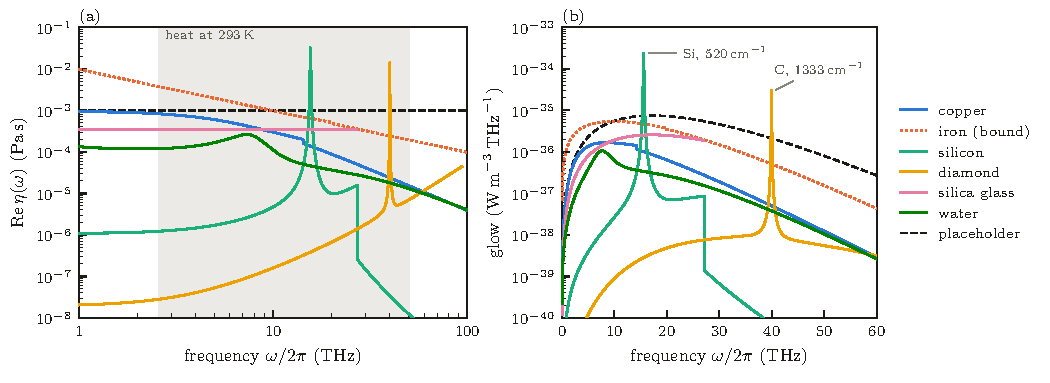
\includegraphics[width=\textwidth]{figures/materials.pdf}
\caption{Gravitational colour. (a) The friction against a uniform shear,
$\mathrm{Re}\,\eta(\omega)$, of the materials of Table~\ref{tab:materials} at
$293\,\mathrm{K}$; the shaded band is where the Planck radiance exceeds a tenth
of its peak. Copper and iron (dotted: the bound for free electrons) relax their
electrons; silicon and diamond have lines at their Raman frequencies, drawn as
damped oscillators of the measured widths whose far wings are not modelled; the
steps are where pair bands end; silica glass is spread evenly over its band;
water's friction rises where its hydrogen bonds stretch. (b) The glow they
send, $4\pi j_\omega$ per unit of frequency, Eq.~\eqref{eq:kirchhoff}, with the
placeholder's for comparison.}\label{fig:materials}
\end{figure*}
